% 原文 p.60（後半）


\subsectionlink{経路情報と環境による監視}
デコヒーレンスに関係する量子力学の形式と解釈の主要要素、すなわち量子状態、重ね合わせ原理、量子もつれ、密度行列、および測定問題を示したので、ついに実際の関心の対象、デコヒーレンスに取り組むための準備が整った。まず、よく知られた二重スリット実験を再訪することによって、この課題に取り組む。この実験は、デコヒーレンスの基本的機構を、非常に直観的で分かりやすく示すだろう。

\subsubsectionlink{二重スリット実験、経路情報、および相補性}
通常の二重スリット装置を描いた図2.2を振り返ろう。左から近づく電子などの粒子が、二つのスリットのあるスクリーンに入射する。スリットを通過した後、遠方の検出スクリーンに当たり、消えない斑点を残す。量子力学が予言し、実験が確認するように、二つの異なる極限的な領域がある（2.2.2節の議論も参照）。
\begin{enumerate}
\item 「波」の状況（図2.2の右）。各粒子がどちらのスリットを通ったかを測定しなければ、検出スクリーンの位置で観測される粒子密度は、$\varrho(x)=\frac12\lvert\psi_1(x)+\psi_2(x)\rvert^2$という干渉模様に対応する。これは、それぞれスリット1、2の通過を表す部分波$\psi_1(x)$、$\psi_2(x)$の、量子力学的重ね合わせに対応する確率密度である。
\item 「粒子」の状況（図2.2の中央）。一方のスリットに検出器を置き、粒子がそのスリットを通ったかを調べると、干渉模様は消える。遠方のスクリーンの密度模様は、スリット1を通ったすべての粒子が作る模様（スリット2を覆ったときに得る模様）と、スリット2を通ったすべての粒子が作る模様を、古典的に足し合わせたもの、$\varrho(x)=\frac12\lvert\psi_1(x)\rvert^2+\frac12\lvert\psi_2(x)\rvert^2$に等しい。
\end{enumerate}

% 原文 p.61
\hypertarget{srcpage:61}{}\label{srcpage:61}
第二の場合、すなわち「粒子」の状況に対する標準的説明は、次のとおりである。量子力学によれば、スリットの位置での粒子の状態は、部分波$\psi_1(x)$、$\psi_2(x)$の重ね合わせ$\Psi(x)=(\psi_1(x)+\psi_2(x))/\sqrt2$で与えられる。この重ね合わせは、両スリットを含む領域に空間的に広がっている。一方のスリットで粒子の位置を測定し、実際にそのスリットに粒子が存在すると分かれば、$\Psi(x)$を対応する空間領域に局在化する。すなわち、$\psi_1(x)$と$\psi_2(x)$は、スリットの位置では重なりが無視できるため、量子力学の標準的な収縮公準を用いて、測定が重ね合わせ$\Psi(x)$を、成分状態$\psi_1(x)$、$\psi_2(x)$の一方へ収縮させたと言える。したがって、部分波間の干渉はもはや得られず、遠方のスクリーンの干渉模様は消える。

言い換えれば、粒子が二つのスリットのどちらを通ったかを見るために、粒子の経路情報（Welcher-Weg情報）を得ようとするたびに、空間的干渉という量子的性質を示す能力を、どうしても破壊してしまうように見える。これは、両スリットを同時に通るという反直観的な事態を記述するように見える、二つの経路の量子力学的重ね合わせを、理解しようとするたびに起こる。したがってNiels Bohrの有名な用語\cite{ref070}を使えば、経路情報（「粒子」の側面）と干渉（「波」の側面）の間には相補性がある。実験設定、すなわち粒子の経路を測定するかどうかに応じて、「粒子的」または「波的」な振る舞いのどちらかを観測するように見える。この「波と粒子の二重性」は量子論の基礎とされ、物理学者と物理哲学者の双方による、数え切れない議論の対象となってきた。

相補性原理とその適用は、1927年にBrusselsで開かれた第5回Solvay会議での、EinsteinとBohrの有名な論争の主題であった\cite{ref071}。Einsteinは会議で、標準的な二重スリット装置についての次の思考実験をBohrに突き付けた。運動量保存則によれば、粒子が上側、または下側のスリットを通ると、スリットを持つスクリーンには、上向き、または下向きの反跳が生じるはずだと論じた。スクリーンの反跳方向を測定できるとしよう（図2.5）。この測定により、少なくとも原理上、粒子の経路を推論でき、経路情報が得られる。Einsteinは、干渉模様はスリットから出る二つの波束の干渉だけによるので、スクリーンの段階で反跳方向を決めても、その後の発展には影響しないはずであり、したがって干渉模様は観測されるはずだと主張した。これはBohrの相補性原理と矛盾するように見える。

% 原文 p.62
\hypertarget{srcpage:62}{}\label{srcpage:62}
\begin{figure}[htbp]\centering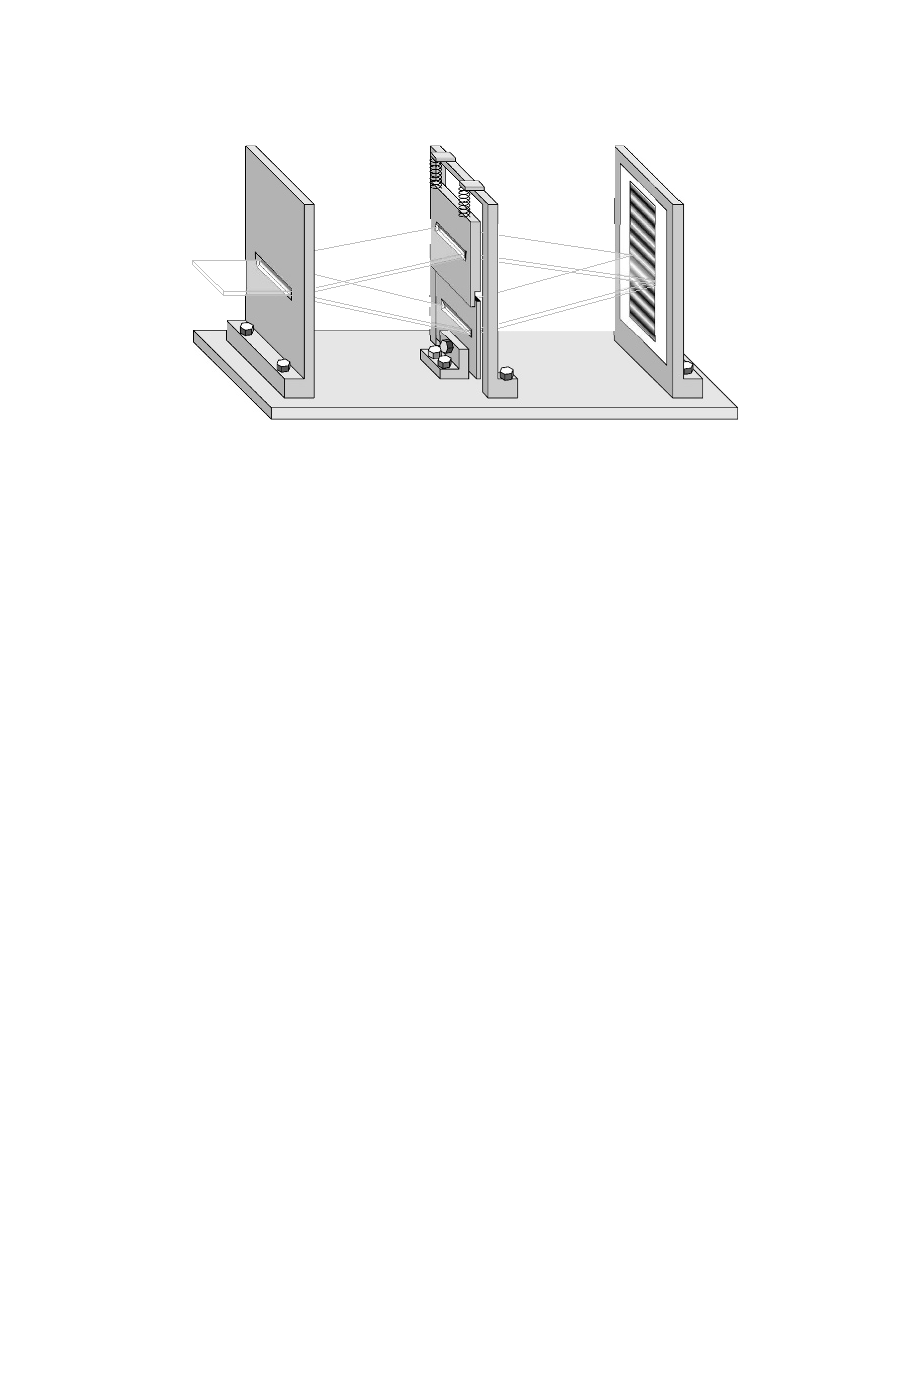
\includegraphics[width=.9\linewidth]{figures/ch02_fig05.pdf}\caption{二重スリット実験で経路情報を得る、Einsteinの思考実験。左のコリメート用スリットを出た粒子は、中央の二重スリットを通り、右の検出スクリーンに記録される。粒子がスリットを通過するとスリットに運動量が伝わり、原理上は、スリットのあるスクリーンの反跳として測定できるはずである。下のスリットは固定し、上のスリットはばねで吊るす。したがって、上のスリットを通る粒子は、吊るされたスリットに小さな振動運動を引き起こし、それを少なくとも原理上は検出できるため、粒子がどちらのスリットを通ったかを推論できる。図はBohrの原図\cite{ref072}に基づき、Macmillan Publishers Ltdの許可により、Nature、copyright 2001の文献\cite{ref073}から転載した。}\end{figure}

Bohrは、この挑戦に次のように応じた。単一粒子がスリットに与える反跳は、通常きわめて小さい。この微小な運動量変化を分解するには、スリットのあるスクリーンの初期運動量を、検出しようとする反跳と少なくとも同じくらい小さな範囲内で知っていなければならない。不確定性原理によれば、スクリーンの運動量をそのような高精度で測定することは、スクリーン位置の大きな不確定性を意味する。そこでBohrは、入射粒子がスリットに到達するより前の、スクリーンの初期運動量の測定だけで、その結果生じる位置の不確定性が、検出スクリーン上の干渉縞の位置に可能な幅を与え、その幅が、干渉縞の特徴的間隔程度になることを示した。したがって、その位置の幅にわたって干渉模様を平均すると、模様は「洗い流される」。ある可能な位置の模様での極大の位置が、別のスクリーン位置に対する模様での極小と重なるので、正味の干渉模様は消える。

% 原文 p.63
\hypertarget{srcpage:63}{}\label{srcpage:63}
したがってBohrの中心的主張は、経路情報の獲得は、不可避な系の擾乱を伴う、というものである。これは、スクリーンの反跳を測って経路情報を得るBohr--Einsteinの例では、実際に正しい。しかし、WoottersとZurek\cite{ref074}が最初に示し、ScullyとDrühl\cite{ref075}がさらに調べたように、ある状況では、粒子の空間波動関数を有意に変化させずに経路情報を集めることもできる。その場合、Bohrが指摘した位置と運動量の不確定性原理の効果は軽減される。次節でこれを論じる。

\subsubsectionlink{量子もつれによる二重スリット実験の記述}
これまで、経路情報の獲得と干渉模様の観測の相補性を、不連続な二者択一の区別として導入した。しかし、たとえば粒子がどちらのスリットを通ったかを不正確に測定して、経路情報の一部だけを集めれば、干渉模様を一部残せないだろうか\cite{ref074}。

この問いの答えは肯定的である。しかし、量子力学のこの特徴を論じ説明するには、上で用いた波動関数の収縮による記述は、もはや適切でない。公準によれば収縮は、不連続で不可逆な過程であり、経路情報量と干渉の程度の、滑らかで可逆な変化を説明できない。代わりに、von Neumann測定方式（2.5.1節）と量子もつれによる、純粋に量子力学的な説明を進める。この記述は、その後、環境が経路検出器の役割を担う、デコヒーレンス過程の記述の基礎にもなる。二重スリット実験での干渉の観測可能性と量子もつれのつながりは、WoottersとZurek\cite{ref074}が初めて論じた。

スリット1、2の通過に対応する粒子の量子状態を、それぞれ$\lvert\psi_1\rangle$、$\lvert\psi_2\rangle$と書こう。前と同じく両方のスリットに検出器を置き、ともに初めは「準備完了」状態にする。スリット2を覆い、粒子源をスリット1のすぐ後ろに置いて粒子が必ずこのスリットを通るようにすれば、粒子を、たとえば状態$\lvert\psi_1\rangle$に準備できる。するとスリット1の検出器は作動し、スリット2の検出器は、作動しない「準備完了」状態にとどまる。以下では、二つの個別検出器を合わせて「検出器」と呼ぶ。この複合検出器の共同の「準備完了」状態を$\lvert\text{「準備完了」}\rangle$、上記のように状態$\lvert\psi_1\rangle$を準備した後の、この検出器系の量子状態を$\lvert1\rangle$と書き、粒子がスリット1を通ったことを示す。この場合、粒子と検出器の複合系の状態発展は、次の形になる。

% 原文 p.64
\hypertarget{srcpage:64}{}\label{srcpage:64}
\begin{equation}\lvert\psi_1\rangle\lvert\text{「準備完了」}\rangle\longrightarrow\lvert\psi_1\rangle\lvert1\rangle.\tag{2.63}\end{equation}
スリットの役割を入れ替えて同じ議論をすると、
\begin{equation}\lvert\psi_2\rangle\lvert\text{「準備完了」}\rangle\longrightarrow\lvert\psi_2\rangle\lvert2\rangle\tag{2.64}\end{equation}
を得る。式(2.63)、(2.64)は、測定相互作用の一般的記述(2.52)に対応する。

両スリットが開いていれば、粒子は二つの成分$\lvert\psi_1\rangle$、$\lvert\psi_2\rangle$の重ね合わせ$\lvert\psi\rangle=(\lvert\psi_1\rangle+\lvert\psi_2\rangle)/\sqrt2$で記述されなければならない。そのため式(2.63)、(2.64)から、von Neumann型(2.54)の力学的発展が得られ、粒子と検出器のもつれた複合状態に至る。
\begin{equation}\frac1{\sqrt2}(\lvert\psi_1\rangle+\lvert\psi_2\rangle)\lvert\text{「準備完了」}\rangle\longrightarrow\frac1{\sqrt2}(\lvert\psi_1\rangle\lvert1\rangle+\lvert\psi_2\rangle\lvert2\rangle).\tag{2.65}\end{equation}
ここでも、検出器状態$\lvert1\rangle$、$\lvert2\rangle$は、系の相対状態$\lvert\psi_1\rangle$、$\lvert\psi_2\rangle$の「指針」として働く。

いま粒子に測定を行うことにより、たとえば位置測定に対応する、検出スクリーンへの衝突によって、粒子について何が分かるだろうか。2.4.6節から分かるように、関心のある量は粒子の縮約密度行列であり、式(2.65)の右辺の純粋状態に対しては、式(2.49)より
\begin{equation}\begin{split}\hat\rho_{\mathrm{particle}}=\frac12\{&\lvert\psi_1\rangle\langle\psi_1\rvert+\lvert\psi_2\rangle\langle\psi_2\rvert\\&+\lvert\psi_1\rangle\langle\psi_2\rvert\langle2\vert1\rangle+\lvert\psi_2\rangle\langle\psi_1\rvert\langle1\vert2\rangle\}.\end{split}\tag{2.66}\end{equation}
この密度行列に対応する、検出スクリーンでの粒子密度$\varrho(x)$は、
\begin{equation}\begin{split}\varrho(x)&\equiv\rho_{\mathrm{particle}}(x,x)\equiv\langle x\rvert\hat\rho_{\mathrm{particle}}\lvert x\rangle\\&=\frac12\lvert\psi_1(x)\rvert^2+\frac12\lvert\psi_2(x)\rvert^2+\operatorname{Re}\{\psi_1(x)\psi_2^*(x)\langle2\vert1\rangle\}\end{split}\tag{2.67}\end{equation}
で与えられる。ここで$\psi_i(x)=\langle x\vert\psi_i\rangle$（$i=1,2$）である。最後の項は、よく知られた干渉模様を記述し、その可視度は重なり$\langle2\vert1\rangle$で定量化されることが分かる。これは、先の2.4.6節の議論に直接につながる。

特に、検出器状態$\lvert1\rangle$、$\lvert2\rangle$が完全に識別可能な極限、$\langle2\vert1\rangle=0$は、「粒子」の領域に対応する。
\begin{equation}\varrho(x)=\frac12\lvert\psi_1(x)\rvert^2+\frac12\lvert\psi_2(x)\rvert^2.\tag{2.68}\end{equation}
逆に、$\lvert1\rangle$、$\lvert2\rangle$が粒子の経路をまったく分解できず、位相因子を無視して$\langle2\vert1\rangle=1$なら、完全な干渉模様という「波」の状況が当てはまる。

% 原文 p.65
\hypertarget{srcpage:65}{}\label{srcpage:65}
\begin{equation}\varrho(x)=\frac12\lvert\psi_1(x)\rvert^2+\frac12\lvert\psi_2(x)\rvert^2+\operatorname{Re}\{\psi_1(x)\psi_2^*(x)\}.\tag{2.69}\end{equation}
検出器が完全ではない一部の経路情報を得る状況は、二つの検出器状態$\lvert1\rangle$、$\lvert2\rangle$の重なりが、非零だが1未満であることで、形式的に表される。式(2.66)から、その場合には干渉模様を観測できるが、重なり$\langle2\vert1\rangle$が小さくなる、すなわち検出器状態$\lvert1\rangle$、$\lvert2\rangle$が識別しやすくなり、検出器が得る経路情報量が増すにつれて、模様は次第に減衰することが分かる。

したがって、経路情報が不完全である限り、干渉模様を観測することと、スリットを通る粒子の経路について、いくらかの情報を得ることは、実際に同時に可能であると示された。検出器の得た情報が、粒子の通った経路を確実に推論できるだけ十分になるとすぐ、干渉模様は消える。WoottersとZurek\cite{ref074}は、経路情報と干渉の、この根本的な相反関係、したがって相補性と量子もつれの密接な関係を分析し、目に見える干渉模様を保ちながら、かなり大量の経路情報を得られることを指摘した。具体的には、経路について90\%の確実さを得ても、干渉模様には約50\%のコントラストが残ることを示した。

まとめると、干渉模様を観測できる程度は、関心のある物体ともつれた、何らかの系に符号化されている、利用可能な経路情報によって決まるだけであり、その量は、必ずしも物体自体の空間波動関数に影響せずに変えられる。したがって相補性は、量子もつれの帰結と見なせる。
